%\documentclass[10pt,a4paper]{article}
\documentclass[12pt,a4paper]{article}

\usepackage[utf8]{inputenc}
\usepackage{hyperref}
\usepackage{polski}
\usepackage{graphicx}
\usepackage{listings}
\usepackage{algorithm}
\usepackage{algorithmic}

\usepackage{hyperref}
%\usepackage{antpolt}
\usepackage{amssymb}
\usepackage{multicol}
\usepackage{fancyvrb}

\usepackage{color}

%\setlength{\topskip}{0mm} \setlength{\footskip}{0mm} \setlength{\topmargin}{0mm} \setlength{\marginparwidth}{0mm}
%\setlength{\headsep}{2mm} \setlength{\headheight}{0mm} \setlength{\textheight}{250mm}
%\setlength{\textwidth}{160mm} \setlength{\oddsidemargin}{0mm} \setlength{\evensidemargin}{0mm}

\setlength{\topskip}{0mm} \setlength{\topmargin}{0mm}
\setlength{\oddsidemargin}{0mm} \setlength{\evensidemargin}{0mm}
\setlength{\marginparwidth}{0mm} \setlength{\headsep}{0mm}
\setlength{\headheight}{0mm} \setlength{\textheight}{240mm}
\setlength{\textwidth}{170mm}


\floatname{algorithm}{Algorytm}
\renewcommand{\lstlistlistingname}{Spis listingów}
\renewcommand{\lstlistingname}{Listing}


% \k{a} \'c \k{e} \l{} \'n \'o \'s
% \'z \.z \k{A} \'C \k{E} \L{} \'N
% \'O \'S \'Z \.Z 

\lstset{literate=
  {á}{{\'a}}1 {é}{{\'e}}1 {í}{{\'i}}1 {ó}{{\'o}}1 {ú}{{\'u}}1
  {Á}{{\'A}}1 {É}{{\'E}}1 {Í}{{\'I}}1 {Ó}{{\'O}}1 {Ú}{{\'U}}1
  {à}{{\`a}}1 {è}{{\`e}}1 {ì}{{\`i}}1 {ò}{{\`o}}1 {ù}{{\`u}}1
  {À}{{\`A}}1 {È}{{\'E}}1 {Ì}{{\`I}}1 {Ò}{{\`O}}1 {Ù}{{\`U}}1
  {ä}{{\"a}}1 {ë}{{\"e}}1 {ï}{{\"i}}1 {ö}{{\"o}}1 {ü}{{\"u}}1
  {Ä}{{\"A}}1 {Ë}{{\"E}}1 {Ï}{{\"I}}1 {Ö}{{\"O}}1 {Ü}{{\"U}}1
  {â}{{\^a}}1 {ê}{{\^e}}1 {î}{{\^i}}1 {ô}{{\^o}}1 {û}{{\^u}}1
  {Â}{{\^A}}1 {Ê}{{\^E}}1 {Î}{{\^I}}1 {Ô}{{\^O}}1 {Û}{{\^U}}1
  {Ã}{{\~A}}1 {ã}{{\~a}}1 {Õ}{{\~O}}1 {õ}{{\~o}}1
  {œ}{{\oe}}1 {Œ}{{\OE}}1 {æ}{{\ae}}1 {Æ}{{\AE}}1 {ß}{{\ss}}1
  {ű}{{\H{u}}}1 {Ű}{{\H{U}}}1 {ő}{{\H{o}}}1 {Ő}{{\H{O}}}1
  {ç}{{\c c}}1 {Ç}{{\c C}}1 {ø}{{\o}}1 {å}{{\r a}}1 {Å}{{\r A}}1
  {€}{{\euro}}1 {£}{{\pounds}}1 {«}{{\guillemotleft}}1
  {»}{{\guillemotright}}1 {ñ}{{\~n}}1 {Ñ}{{\~N}}1 {¿}{{?`}}1
  {ł}{\l{}}1 {ś}{{\'s}}1 {ź}{{\.z}}1  {ó}{{\'o}}1
}

\begin{document}
\pagestyle{empty}

%
%  strona tytułowa
%

\begin{center}
\textsc{\Huge{Uniwersytet Zielonogórski}}\\
\LARGE{Wydział Informatyki, Elektrotechniki i Automatyki}\\
\vspace{0.5cm}
\Large{Platforma .NET -- Projekt}\\
Prowadzący: dr inż. Marek Sawerwain\\ \vspace{1cm}
\LARGE{Tytuł raportu/sprawozdania}\\
\vspace{0.5cm} 
\Large{Wykonał: Damian Radecki, Grupa dziekańska: 33-INF-SSI-SP} \\
\Large{Projekt realizowano razem z: \\ Damian Kurkiewicz}\\
\Large{Data oddanie projektu: DD mmmm YYYY}
\vspace{1cm}
\begin{flushleft}
	Ocena: ..........................................
\end{flushleft}
\vspace{1cm}
\end{center}



%
% spis treści
%

\begin{multicols}{2}
	\footnotesize
	\tableofcontents
\end{multicols}


%
% spis listingów
%

\begin{multicols}{2}
	\footnotesize
	\lstlistoflistings
\end{multicols}




\noindent\makebox[\linewidth]{\rule{0.6\paperwidth}{0.4pt}}

\begin{flushleft}
	\emph{Motto:}\\
	\textit{Pisanie raportu przywilejem każdego studenta.}
\end{flushleft}

% 1. Wprowadzenie
% 2. Użyte technologie
% 3. Projekt i implementacji
% 4. Testy (jednostkowe, testy UI)
% 5. Wdrożenie -- instalacja
% 6. Wkład poszczególnych Autorek/Autorów projektu
% 7. Podsumowanie


\section{Wprowadzenie} 

\subsection{Aplikacje czasu rzeczywistego}
\hspace*{0.7cm} Aplikacje działające na żywo oferują wiele korzyści, które są sporym ułatwieniem dla użytkowników podczas używania takiej aplikacji. Czynności wykonywane
bez odświeżania strony nie tylko skracają czas wykonywania czynności czy obsługiwania samej witryny to jeszcze znacznie ułatwiają komunikację, unikają 
blokowania strony i tworzą bardziej intuicyjny interface. Takie aplikacje internetowe staja się normą w dzisiejszych czasach. Każde przeładowanie strony jest
nie komfortowe i stwarza pewnego rodzaju niebezpieczeństwo wykradnięcia danych. Serwisy internetowe obsługujące komunikację real-time z klientem są lepiej 
zabezpieczone i działają wydajnościowo lepiej. Powstawało wiele technologii do wsparcia komunikacji na żywo, które działają zarówno po stronie witryny i
serwera. Są to między innymi \textit{WebSocket, SignalR, RabbitMQ czy Apache Kafka}. Wszystkie z nich są dziś globalnie używane do wsparcia przekazu informacji.

\subsection{Opis działania}
\hspace*{0.7cm} Projekt chatu na żywo jest aplikacją, która wspiera komunikację między użytkownikami, aby ich konwersacje nie działały w stylu w jakim działa klasyczny serwer
e-mail. Założenie projektu są takie, aby użytkownicy bez przeładowania strony mogli wymieniać miedzy sobą wiadomości. Dodatkowo wszelkie powiadomienia
przychodzą również bez zbędnego odświeżania witryny. Sprawia to, że witryna jest bardziej intuicyjna, łatwiejsza i szybsza w obsłudze. Taka architektura
aplikacji jest przyjazna użytkownikowi, od którego będzie wymagana minimalny wysiłek w trakcie używania strony. Celem takiej aplikacji jest też maksymalne 
bezpieczeństwo wspierane przez bearen token i autoryzację użytkowników z zachowaniem szyfrowania danych poufnych. Architektura zapewnia, że nie będziemy otrzymywać wiadomości od niezaakceptowanych użytkowników lecz daje możliwość uczestnictwa w czatach posiadających osoby nieznajome poprzez mechanizm grup. W grupach każdy użytkownik może zaprosić swoich znajomych co może spowodować komunikację między nieznajomymi w danym czacie.


\subsection{Grupa docelowa}
\hspace*{0.7cm} Grupą docelową są wszyscy użytkownicy którzy cenią sobie bezpieczeństwo i wygodę. Chcą szybko skomunikować się ze swoimi przyjaciółmi bądź grupą docelową
bez żadnych opóźnień czy niepotrzebnych przeładować strony. Są pewni tego, że ich dane są przechowywane w bezpiecznym miejscu i nikt nie wkradnie się na ich
konto. Mogą to być zarówno firmy, które chcą komunikować się między sobą i ewentualnie z klientami poprzez utworzenie chatu dla grupy użytkowników jak i dla szkół, uniwersytetów, grup pracowników, przyjaciół czy kolegów. 


\section{Użyte technologie}

\subsection{.Net Core} 			%razem
\hspace*{0.7cm} Popularny, nowoczesny i wydajny framework oparty o otwartoźródłowa implementację, który został wydany w 2016 roku do ogólnego przeznaczenia. Stanowi zestaw bibliotek pozwalający tworzyć wieloplatformowe aplikacje o wysokim stopniu bezpieczeństwa. Framework ten pozwala na pisanie aplikacji między innymi przeznaczonych do obliczeń chmurowych, IoT oraz jak w naszym przypadku do pisania web serwisu. 

\begin{figure}[H]
	\centering
	
\includegraphics[width=0.3\linewidth]{dotnet5_platform}
	\caption{Logo .Net Core}
	\label{fig:dotnet5platform}
\end{figure}

Framework \textit{.Net Core} został przez nas wybrany, ponieważ jest to nowa oraz dobrze prosperująca technologia wprowadzająca dużą dawkę świeżości podczas tworzenia nowego oprogramowania. Posiada wsparcie dla tworzenia web serwisów opartych o metodykę \textit{REST}, poprzez dodanie nowych i gotowych do działania bibliotek. Platforma \textit{.Net Core} jest znacznie wydajniejsza od .Net Framework. Wprowadza znaczące usprawnienia przekładające się na szybkość działania pisanych programów. Architektura przedstawia się w sposób następujący.\newline

\begin{figure}[H]
	\centering
	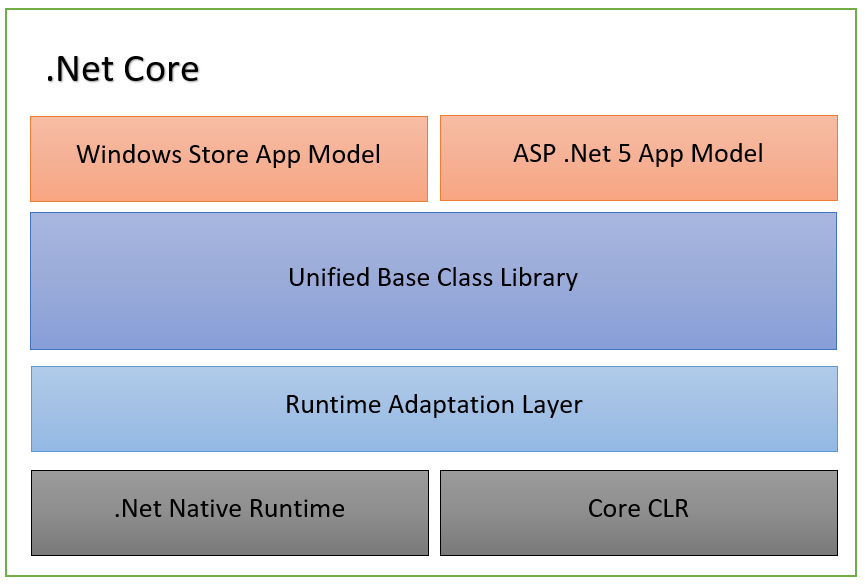
\includegraphics[width=0.7\linewidth]{net-Core-1}
	\caption{Architektura .NET Core}
	\label{fig:net-core-1}
\end{figure}

\subsection{Entity Framework}   %ja

\hspace*{0.7cm} \textit{Entity Framework} to zestaw technologii \textit{ADO.NET}, obsługujące opracowywanie aplikacji zorientowanych na dane. Framework ten pozwala modelować konkretne jednostki, relację czy też logikę działania bazy danych. Obsługuję wiele systemów magazynowania danych takich jak na przykład \textit{MySQL}, który to został przez nas wybrany do realizacji projektu. Całość jest konfigurowalna z poziomu kodu co jest bardzo wygodnym rozwiązaniem. Pozwala deweloperom na współpracę z danymi w postaci obiektów. Model fizyczny jest rafinowany przez administratorów bazy danych w celu zwiększenia wydajności, ale programiści piszący kod aplikacji przede wszystkim zawężają się do pracy z modelem logicznym, pisząc zapytania \textit{SQL} i wywołując procedury składowane. Modele domen są zwykle używane jako narzędzie do przechwytywania i komunikowania się z wymaganiami aplikacji, często tak jak w przypadku diagramów obojętnych, które są wyświetlane i omówione w wczesnych etapach projektu, a następnie porzucone. Wiele zespołów programistycznych pomija Tworzenie modelu koncepcyjnego i rozpoczyna się od określenia tabel, kolumn i kluczy w relacyjnej bazie danych.\newline

\begin{figure}[H]
	\centering
	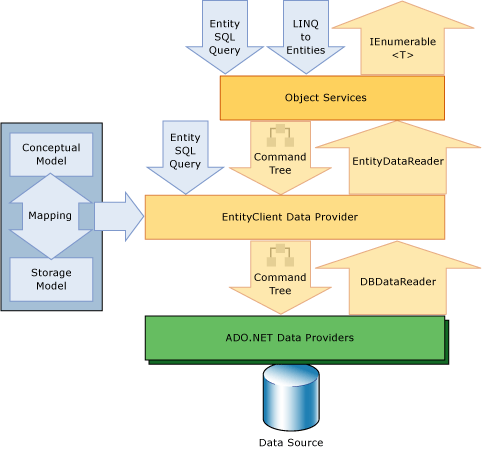
\includegraphics[width=0.7\linewidth]{entity}
	\caption{Architektura Entity Framework do uzyskania dostępu do danych}
	\label{fig:entity}
\end{figure}


\subsection{SignalR} 			%kurek

\hspace*{0.7cm} Biblioteka dla dewelpoarów \textit{ASP.NET}, która przyśpiesza proces dodawania funkcji sieci web w czasie rzeczywistym do aplikacji. Często wykorzystuje się tą bibliotekę w czatach internetowych, lecz może ona o wiele więcej. \textit{SignalR} może być używany też w takich aplikacjach jak pulpity nawigacyjne, aplikacje do monitorowania czy formularze działające w czasie rzeczywistym. Biblioteka umożliwia również zupełnie nowe typy aplikacji internetowych, które wymagają aktualizacji wysokiej częstotliwości z serwera, na przykład gier w czasie rzeczywistym.
Komunikacja między stroną a serwerem odbywa się poprzez tak zwane Hub'y. Bardzo dobrze ukazuje to rysunek poniżej. \newline

\begin{figure}[H]
	\centering
	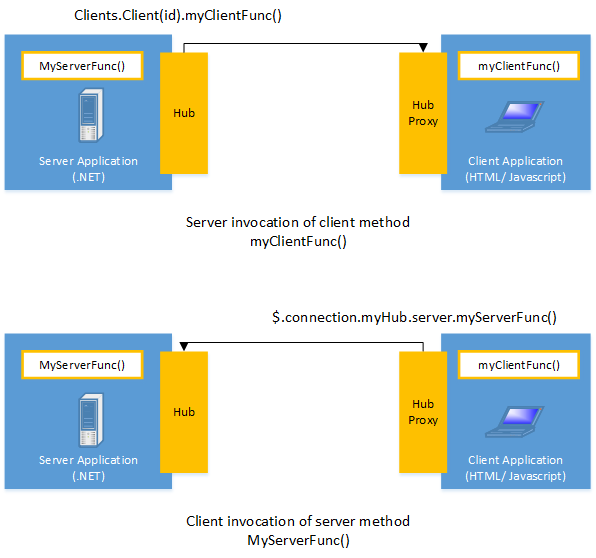
\includegraphics[width=0.7\linewidth]{signalr}
	\caption{SignalR przykład działania}
	\label{fig:signalr}
\end{figure}

\subsection{MySql} 				%ja

\hspace*{0.7cm} Baza danych rozwijana przez firmę \textit{Oracle}. \textit{MySql} jest to otwarto źródłowy system zarządzania relacyjnymi bazami danych. System ten obsługuję język zapytań \textit{SQL}, który służy do pisania zapytań do tej bazy. \textit{MySql} jest relacyjną bazą danych. Model relacyjny w prosty i intuicyjny sposób przedstawia dane w tabelach. Każdy wiersz w tabeli jest rekordem z unikatowym identyfikatorem zwanym kluczem. Kolumny tabeli zawierają atrybuty danych, a każdy rekord zawiera zwykle wartość dla każdego atrybutu, co ułatwia ustalenie relacji między poszczególnymi elementami danymi.\newline
 
\begin{figure}[H]
	\centering
	
\includegraphics[width=0.7\linewidth]{mysql-logo}
	\caption{Logo MySQL}
	\label{fig:mysql-logo}
\end{figure}

\subsection{Angular} 			%kurek

\hspace*{0.7cm} Otwarto źródłowy framework \textit{JavaScript}, zaprojektowany i napisany przez inżynierów z \textit{Google}. Ich celem było zrewolucjonizowanie projektowania części wizualnej stron internetowych. Szybko zyskał popularność wśród programistów JavaScript, którzy zaczęli odstawiać go na rzecz \textit{jQuery}. Jego największą zaletą oraz najbardziej rozpoznawalną cechą jest integracja z atrybutami \textit{HTML}. Framework ten umożliwia proste wdrożenie wzorca \textit{MVC(Model-View-Controller)}, dzięki czemu testowanie jak i rozwój aplikacji nie sprawia wielu problemów.

\begin{figure}[H]
	\centering
	
\includegraphics[width=0.7\linewidth]{AngularJS_logo}
	\caption{Logo Angular}
	\label{fig:angularjslogo}
\end{figure}


\section{Projekt}

\subsection{Struktura projektu} %razem

\hspace*{0.7cm} Diagram pokązujący architekturę całego projektu opisuje główne komponenty i występujące między nimi połączenia. Strona internetowa napisana w Angularze jest podłączona bezpośrednio z \textit{SignalR} i web serwisem. Miedzy nim występują połączenia dwukierunkowe. Z tym pierwszym strona internetowa utrzymuje stałe połączenie, aby zapewnić natychmiastową wymianę danych. Drugi wymieniony komponent odpowiada na zadane żądania. \textit{SignalR} został wbudowany w web serwis jako integralna część, ale jest traktowany osobno, ponieważ utrzymuje z klientem innego typu połączenie. Między nimi także następuje wymiana danych. Ostatnim komponentem projektu jest baza danych, która jest podłącza tylko do web serwisu. To on stanowi most do pobierania wszelkich zawartych tam informacji. 

\begin{figure}[H]]
	\centering
	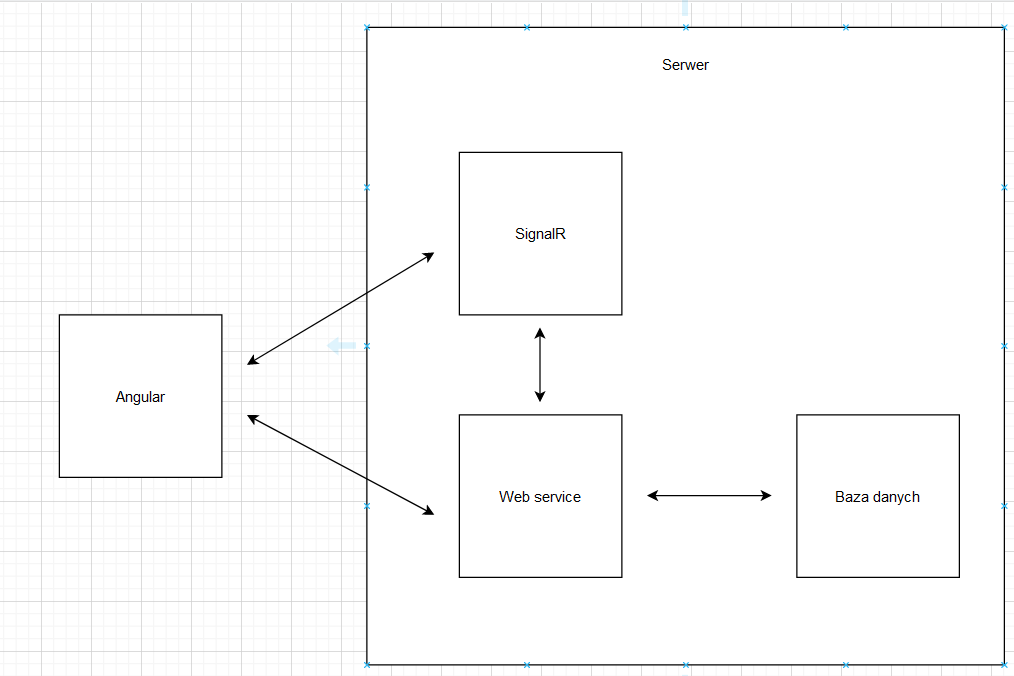
\includegraphics[width=0.7\linewidth]{diagramProjektu}
	\caption{}
	\label{fig:diagramprojektu}
\end{figure}
			
\subsection{Diagram Gantta}				%razem

\hspace*{0.7cm} Diagram Gantta dla naszego projektu przedstawia się następująco:

\begin{figure}[H]
	\centering
	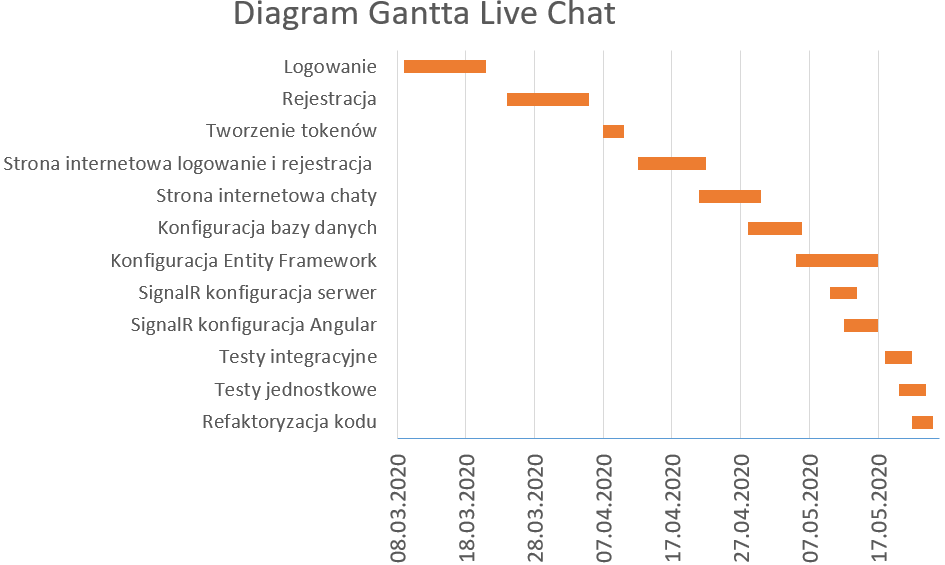
\includegraphics[width=0.8\linewidth]{diagramGantta}
	\caption{Diagram Gantta Live Chat}
	\label{fig:diagramgantta}
\end{figure}

\subsection{Use Cases}					%razem
\hspace*{0.7cm} Use case pokazują fukcjonalności projektu z podziałem na rodzaje użytkownik danej aplikacji. W live chat bedziemy wyrózniać dwa rodzaje użytkowników. Będzie to nowy user, który będzie miał możliwość jedynie rejestracji i drugi to będzie już utworzony user, który będzie mógł korzystać ze wszystkich korzyści programu.

\begin{figure}[H]
	\centering
	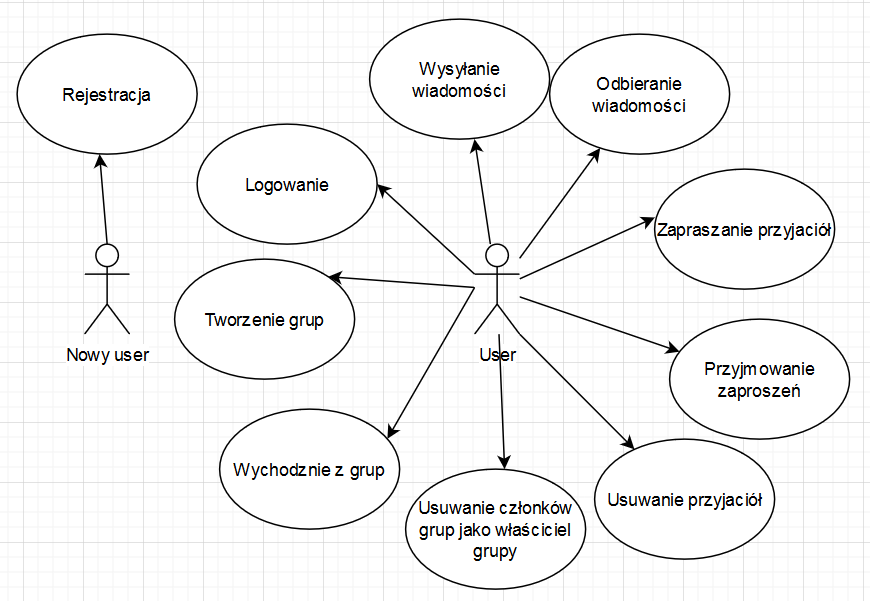
\includegraphics[width=0.7\linewidth]{usecase}
	\caption{}
	\label{fig:usecase}
\end{figure}

\subsection{Struktura bazy danych}  	%ja
\hspace*{0.7cm} Struktura bazy danych jest prosta i czytelna. Dla takiego projektu baza danych jest fundamentem. Musimy mieć miejsce do przechowywania informacji o użytkownikach, relacjach, wiadmościach czy czatach. Tabele opieraja się na relacjach między sobą. Sama struktura w mysql została wygenerowana przez \textit{Entity Framework Core}, który zrobił w najbardziej optymalny i wydajny sposób.

\begin{figure}[H]
	\centering
	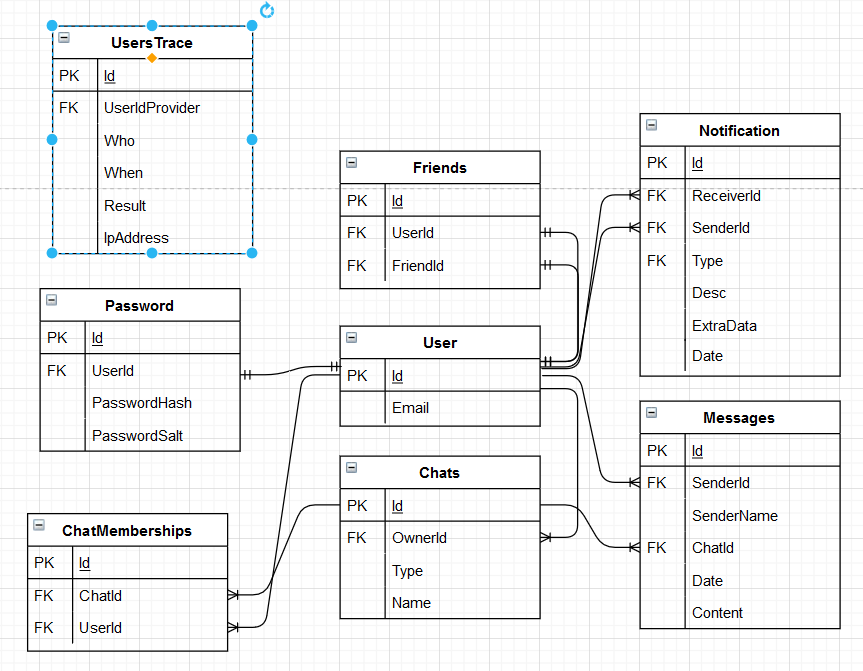
\includegraphics[width=0.7\linewidth]{diagrambazydanycj}
	\caption{}
	\label{fig:diagrambazydanycj}
\end{figure}


\subsection{Komunikacja z web serwisem} %kurek
\hspace*{0.7cm} Komunikacja z web serwisem została podzielona na część dla każdego usera i część tylko dla zalogowanych.
Po zalogowaniu wytwarzany jest token w \textit{User Controller} i przesyłany z powrotem do klienta. Takowy token jest wykorzystywany do autoryzacji podczas dostępu do pozostałych kontrolerów. W przypadku \textit{SignalR}, tylko zalogowani użytkownicy mogą się podłączyć. Wywoływana jest metoda RPC do walidacji użytkownika. Jest to druga część autoryzacji co czyni ją dwuetapową. Ta część polega na sprawdzeniu czy email zawarty w tokenie zgadza się z id usera. Wywoływana jest wówczas baza danych do pobrania emailu zawartego w rekordzie o danym id i przyrównanie tej wartości z wartością email zawartą w tokenie. Prosty diagram komunikacji z web serwisem jest następujący.

\begin{figure}[H]
	\centering
	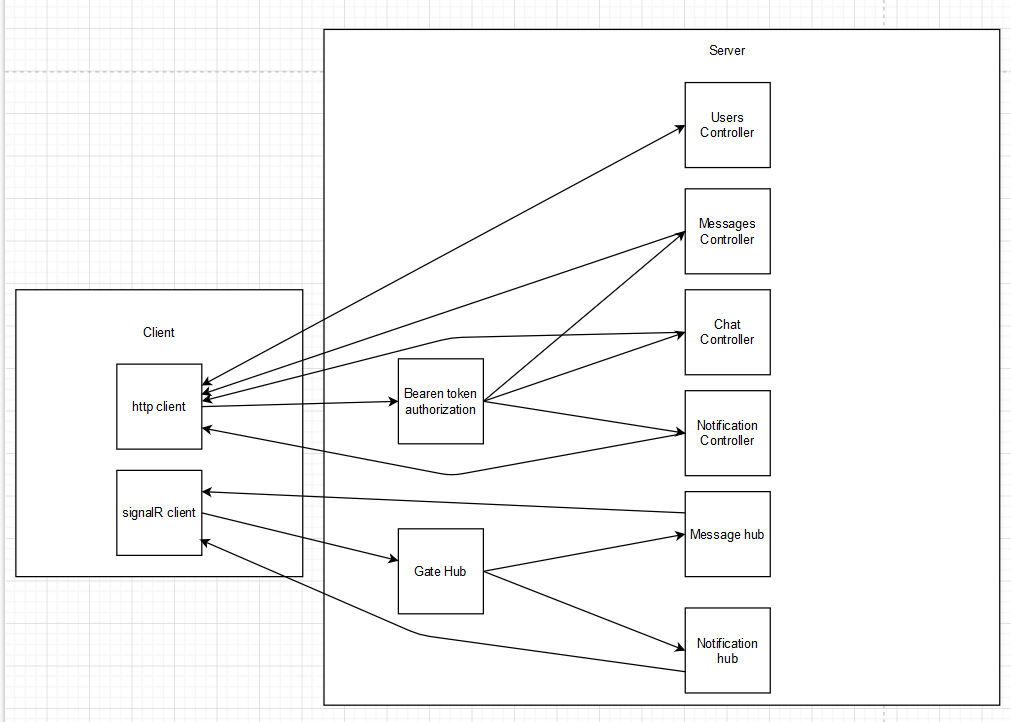
\includegraphics[width=1\linewidth]{komunikacjazwebserwisem}
	\caption{}
	\label{fig:komunikacjazwebserwisem}
\end{figure}


\subsection{Diagram klas}
\hspace*{0.7cm} Diagram klas przedstawia od strony czysto technicznej połączenia między poszczególnymi klasami, interfejsami czy typami prostymi. Pozwala zauważyć pewne założenia, schematy, które ułatwią implementowanie całego mechanizmu, aby uniknąć powtarzania się kodu czy zminimalizować ilość użytych linijek. 

%\begin{figure}[H]
%	\centering
%	\includegraphics[width=1\linewidth]{C:/Users/ditri/Downloads/DiagramKlas(2)}
%	\caption{}
%	\label{fig:diagramklas2}
%\end{figure}

\section{Implementacja}

\subsection{Modele bazy danych}				%ja - enity framework

\hspace*{0.7cm} Baza danych dla naszego projektu musiała być bardzo rozbudowana. W trakcie samego tworzenia, modeli ciągle przybywało. Jako że używaliśmy Entity Frameworka zdecydowaliśmy się na użycie adnotacji dla klas modeli. Skorzystaliśmy z bibliotek \textit{System.ComponentModel.DataAnnotations}. Jedenym z przykładowych lecz bardziej rozbudowanych modeli użytych w naszej bazie danych znajduje się na listingu poniżej, dana klasa została przygotowana dla tabeli zawierającej wiadomości.\newline

\begin{lstlisting}[caption={Przykładowa klasa modelu tabeli - Message}]

	public class Message
	{
	 	[Key]
	 	public int Id { get; set; }
		
		[Required]
		[ForeignKey("Sender")]
		[JsonIgnore]
		public int SenderId { get; set; }
		
		[JsonIgnore]
		public virtual User Sender { get; set; }
		
		public string SenderName { get; set; }
		
		[Required]
		[ForeignKey("Chat")]
		public int ChatId { get; set; }
		
		[JsonIgnore]
		public virtual Chat Chat { get; set; }
		
		public DateTime Date { get; set; }
		
		public string Content { get; set; }
	}
	
\end{lstlisting}

\hspace*{0.7cm} Jak widać na powyższym listingu. Model ten zawiera takie adnotacje:
\begin{itemize}
	\item \textbf{Key} - określa że dane pole jest kluczem głównym;
	\item \textbf{Required} - informuje żę dane pole musi być wypełnione;
	\item \textbf{ForeignKey} - oznacza daną zmienną jako klucz obcy oraz w nawiasie przyjmuje nazwę tabeli której jest to klucz obcy;
	\item \textbf{JsonIgnore} - adnotacja wskazuje że dane pole bądź metodę należy zignorować podczas deserializacji danych.
\end{itemize}

\subsection{Modele DTO} 					%kurek
\hspace*{0.7cm} \textit{Model DTO (Data Transfer Object)}  jest bardzo wygodnym wzorcem projektowym należącym do grupy wzorców dystrybucji. Dzięki DTO można w prosty sposób transferować dane między systemami czy aplikacjami. W naszym projekcie potrzebowaliśmy stworzyć wiele modeli DTO w celu komunikacji \textit{Strona web - Serwer}. Dobrze skonstruowany kontener, bo tak często nazywana jest klasa będąca modelem DTO, często staje się podstawową konstrukcją w wielu rozbudowanych projektach. W naszym projekcie znajduję się aktualnie aż osiem modeli DTO. Posiadamy modele potrzebne do transportu wiadomości czy też powiadomień. Jak wygląda przykładowy model DTO użyty w naszym projekcie znajduje się poniżej:\newline

\begin{lstlisting}[caption={Przykładowa klasa modelu DTO - Message}]

public class InvitatationDTO
{
 [Required]
 [RegularExpression(@"^[1-9]\d*$", ErrorMessage = "'0' Can not be used")]
 public string UserId { get; set; }
	
 [Required]
 [RegularExpression(@"^[1-9]\d*$", ErrorMessage = "'0' Can not be used")]
 public string OtherId { get; set; }
	
 public string ChatId { get; set; }
}
\end{lstlisting}

\hspace*{0.7cm} Powyższy listing pokazuje że w projekcie użyliśmy również wyrażeń regularnych w celu sprawdzania poprawności przesyłanych danych. W momencie gdy przesłany przez stronę \textit{Model DTO} zawiera dane nie zgodne z wyrażeniem regularnym, serwer automatycznie zwracał błąd że jakieś dane są nie poprawne. Dzięki temu mogliśmy pominąć sprawdzanie wielu przypadków przesyłania błędnych danych.


\subsection{Implementacja kontrolerów}		%razem
\subsection{Problemy i ich rozwiązania}		%razem

\section{Testy}

\subsection{Testy jednostkowe}   %ja
\subsection{Testy integracyjne}  %kurek

\section{Opis wkładu własnego w realizację projektu}

%ja
\subsection{Stworzenie i konfiguracja bazy danych}

\hspace*{0.7cm} Złożoność oraz poziom zaawansowania naszego projektu był bardzo duży co wymagało rozbudowanej bazy danych. Budowę oraz połączenie między tabelami w bazie danych ukazuje rysunek numer \ref{fig:diagrambazydanycj}. Praktycznie każda tabela posiada klucz obcy innej tabeli. Spowodowane to jest tym iż specyfika naszego projektu wymaga od nas takiego połączenia. Każdy czat musi być przypisany do konkretnych użytkowników, każda wiadomość do konkretnego czatu. Powiadomienia w podobny sposób co wiadomości czy czaty muszą posiadać przypisanego konkretnego użytkownika, a do tego wszystkiego jeszcze dochodzą czaty grupowe co wymagało od nas dodatkowego przemyślenia działania całej infrastruktury aplikacji.\newline

\hspace*{0.7cm} Po wielu problemach i próbach ich rozwiązania udało nam się skonfigurować \textit{Entity Framework} do oczekiwanego przez nas stopnia. Większość tabel i połączeń między nimi bardzo dobrze się skonfigurowało poprzez adnotacje nadane polom w modelach bazy danych. Sam nasz \textit{DbContext} wyglądał w sposób następujący:\newline

\begin{lstlisting}[caption={DbContext Entity Framework}]

public DbSet<Password> Passwords { get; set; }
public DbSet<User> Users { get; set; }
public DbSet<Message> Messages { get; set; }
public DbSet<Relation> Friends { get; set; }
public DbSet<Notification> Notifications { get; set; }
public DbSet<Chat> Chats { get; set; }
public DbSet<ChatMembership> ChatMemberships { get; set; }
public DbSet<UserTrace> UsersTrace { get; set; }

\end{lstlisting}

\hspace*{0.7cm} Powyższa część odpowiada za utworzenie tabel \textit{DBSet} z nazwą modelu we wnętrzu trójkątnych nawiasów. Niestety nie wszystkie tabele chciały się w ten sposób utworzyć. Jedyną tabelą, którą musieliśmy utworzyć w trochę inny sposób okazała się tabela \textit{Notyfication} odpowiadająca za przetrzymywanie informacji na temat powiadomień. Tą jedną tabelę utworzyliśmy używając wbudowanych dodatkowych funkcji \textit{Entity Frameworka}, nadpisując funkcję \textit{OnModelCreating} byliśmy w stanie utworzyć tabelę wraz jej połączeniami. Poniższy listing ukazuje naszą rozbudowę funkcji:\newline

\begin{lstlisting}[caption={OnModelCreating tabela Notyfication - Entity Framework}]

protected override void OnModelCreating(ModelBuilder modelBuilder)
{
	base.OnModelCreating(modelBuilder);
	
	modelBuilder.Entity<Notification>()
	.HasOne(t => t.Sender)
	.WithMany(m => m.NotificationsSent)
	.HasForeignKey(p => p.SenderId);
	
	modelBuilder.Entity<Notification>()
	.HasOne(t => t.Receiver)
	.WithMany(m => m.NotificationsReceived)
	.HasForeignKey(p => p.ReceiverId);
}
\end{lstlisting}

\subsection{Stworzenie systemu logowania i rejestracji}

\hspace*{0.7cm} Stworzenie przez nas systemu logowania i rejestracji było bardzo skoplikowanym procesem. Przemyśleć musieliśmy jakiego algorytmu szyfrowania haseł użyć by hasła użytkowników przechowywane w bazie danych były bezpieczne. Do szyfrowania haseł użyliśmy wbudowanego w język \textit{C\#} algorytmu wyznaczania wartości skrótu zwangeo \textit{HMAC-SHA512}, który to zbudowany jest z funkcji skrótu \textit{SHA-512} oraz oparty jest o uwierzytelnianie wiadomości opartych o skróty \textit{HMAC}. Proces \textit{HMAC} miesza klucz tajny z danymi komunikatów i miesza wynik. Wartość skrótu jest ponownie mieszana z kluczem tajnym, a następnie poddana skrótu po raz drugi. Wynikowy skrót ma długość 512 bitów.\textit{HMAC} działa w sposób następujący:\newline

\begin{figure}[H]
	\centering
	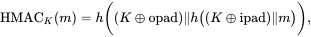
\includegraphics[width=0.7\linewidth]{hmac_signature}
	\caption{HMAC Signature}
	\label{fig:hmac_signature}
\end{figure}

\hspace*{0.7cm} Podczas rejestracji szyfrowane jest hasło po stronie serwera oraz zaszyfrowane zapisywane jest w bazie danych. W celu zapobiegnięcia odszyfrowania, hasło jest szyfrowane w jedną stronę. Dzięki temu nawet my jako twórcy nie jesteśmy w stanie od szyfrować dla własnych potrzeb hasła użytkownika. Logowanie przeprowadza podobny proces co rejestracja lecz nie zapisuje hasła w bazie. Hasło wpisane przez użytkownika jest szyfrowane po stronie serwera i już zaszyfrowane hasło jest porównywane z zaszyfrowanym hasłem w bazie danych. Jeśli wartości są takie same użytkownik zostaje poprawnie zarejestrowany w aplikacji i uzyskuje dostęp do wszystkich funkcji systemu.

\subsection{Autoryzacja i autentykacja użytkowników}

\hspace*{0.7cm} W celu autoryzacji oraz autentykacji użytkowników po stronie serwera. Tworzony jest token. Token jest to ciąg znaków identyfikujący aktualnie zalogowanego użytkownika. Tworzony jest w taki sposób by nie było możliwości powtórzenia się tokena.

\begin{lstlisting}[caption={Tworzenie tokena przy logowaniu}]]

var tokenDescriptor = new SecurityTokenDescriptor
{
	Subject = new ClaimsIdentity(claims),
	Expires = DateTime.Now.AddHours(12),
	SigningCredentials = creds
};

var tokenHandler = new JwtSecurityTokenHandler();
var token = tokenHandler.CreateToken(tokenDescriptor);

\end{lstlisting}

\hspace*{0.7cm} Jak widać na powyższym listingu, do tworzenia tokena uwierzytelniającego użytkownika wykorzystujemy klasę \textit{SecurityTokenDescriptor}. Dzięki tej klasie jesteśmy w stanie przekazać jej wszystkie potrzebne informacje do utworzenia tokena. Token jest ważny przez 12 godzin ale jeśli użytkownik zamknie kartę z otwarta naszą stroną automatycznie token jest usuwany. Natomiast gdy użytkownik przekroczy czas dwunastu godzin zostanie poproszony o ponowne zalogowanie. Po utworzeniu tokena przesyłamy w formacie \textit{JSON} token wraz z informacjami o zalogowanym użytkowniku do aplikacji w przeglądarce.

\subsection{Konfiguracja środowiska i serwera}

\hspace*{0.7cm} Konfiguracja aplikacji rozrastała się w raz z powstawaniem nowych funkcji. Przed rozpoczęciem działania aplikacji odpalana jest konfiguracja, która trzeba najpierw skonfigurować. Klasa \textit{Startup} metody takie jak \textit{ConfigureService} oraz \textit{Configure}. Zacznijmy od tej pierwszej. Metoda \textit{ConfigureServices} jest metodą opcjonalną. Wywoływana jest przez hosta przed uruchomieniem metody \textit{Configure}. W metodzie tej wszystkie opcje konfiguracyjne ustawiane są wraz z konwencją przedstawianą w dokumentacji firmy.

\subsubsection{ConfigureServices}

\hspace*{0.7cm} W tej metodzie jako pierwsze ustawiamy dostęp do bazy danych oraz wskazujemy do jakiej bazy chcemy się łączyć. W naszym przypadku łączymy się do bazy \textit{MySQL}.

\begin{lstlisting}[caption={Dodanie bazy danych do konfiguracji}]
services.AddDbContext<DataContext>(option => 
{
 option.UseLazyLoadingProxies();
 option.UseMySql(Configuration.GetConnectionString("DefaultConnection"));
});
\end{lstlisting}

\hspace*{0.7cm} \textit{ConnectionString} jest pobierany z pliku konfiguracyjnego. Opcja \textit{UseLazyLoadingProxies} powoduje tak zwane Leniwe Ładowanie, które polega na każdorazowym odpytywaniu bazy o interesujące nas dane. Ten typ ładowania jest wykorzystywany gdy chcemy pobrać jakieś konkretne dane z bazy a nie chcemy zaśmiecać sobie pamięci masą innych niepotrzebnych danych.\newline

\hspace*{0.7cm} Jako drugie ustawiamy zakres. Zakresy są potrzebne do bazy danych. Informujemy w ten sposób które interfejsy oraz klasy należą do kontroli bazy danych. Dodajemy je w następujący sposób:

\begin{lstlisting}[caption={Dodanie klas Repository}]
services.AddScoped<IUserRepository, UserRepository>();
services.AddScoped<INotificationRepository, NotificationRepository>();
services.AddScoped<IMessagesRepository, MessageRepository>();
services.AddScoped<IChatRepository, ChatRepository>();
\end{lstlisting}

\hspace*{0.7cm} Powyższy listing przedstawia w jaki sposób dodajemy klasy oraz interfejsy, które są repozytoriami dla danych tabel w bazie danych.\newline

\hspace*{0.7cm} Następną częścią jaką dodajemy do naszej konfiguracji są wzorce projektowe \textit{Singleton}. \textit{.Net Core} posiada wbudowane metody pozwalające na tworzenie konkretnych klas na serwerze jako \textit{Singletony}. W jaki sposób to się robi przedstawia poniższy listing z naszego programu:

\begin{lstlisting}[caption={Wzorzec Singleton w konfiguracji}]
services.AddSingleton<MessageConnectionService>();
services.AddSingleton<NotificationConnectionService>();
services.AddSingleton<Func<ServiceTypes, IConnectionService>>(provider => serviceType =>
{
	switch(serviceType)
	{
	case ServiceTypes.MessageConnectionService:
		return provider.GetService<MessageConnectionService>();
	case ServiceTypes.NotificationConnectionService:
		return provider.GetService<NotificationConnectionService>();
	default:
		return null;
	}
});
\end{lstlisting}

\hspace*{0.7cm} Kolejną bardzo ważną częścią jak nie najważniejszą w konfiguracji jest autentykacja i autoryzacja. W naszej aplikacji użyliśmy tak zwanego \textit{BearerTokena}. Określamy wszelkie ustawienia jego jak i to jakim kluczem jest szyfrowane oraz podajemy token potrzebny do tworzenia klucza. Tak jak w przypadku \textit{ConnectionString} tutaj pobierana jest wartość z pliku zawierającego dane konfiguracyjne. Poniższy listing przedstawia jak skonfigurowany jest nasz \textit{BearerToken}.

\begin{lstlisting}[caption={BearerToken - konfiguracja}]
services.AddAuthentication(JwtBearerDefaults.AuthenticationScheme)
 .AddJwtBearer(options =>
 {
 options.TokenValidationParameters = new TokenValidationParameters
 {
  ValidateIssuerSigningKey = true,
  IssuerSigningKey = new  SymmetricSecurityKey(Encoding.ASCII.GetBytes(
  Configuration.GetSection("AppSettings:Token").Value)),
  ValidateIssuer = false,
  ValidateAudience = false,
 };
 options.Events = new JwtBearerEvents
 {
  OnMessageReceived = context =>
  {
   var accessToken = context.Request.Query["access_token"];
  if (string.IsNullOrEmpty(accessToken) == false)
  {
   context.Token = accessToken;
  }
   return Task.CompletedTask;
  }
 };
});
\end{lstlisting}    

\hspace*{0.7cm} Ostatnią częścią tej metody jest dodanie tak zwanej \textit{Policy}. Ta część pozwala na ustawienie metod, nagłówków oraz ustawienie jaki adres jest tym domyślnym, bazowym. W naszym przypadku jako że to projekt, adres bazowy posiada u nas wartość \textit{http://localhost:4200}. Na sam koniec dodajemy obsługę bibliotek \textit{SingalR}. Poniższy listing przedstawia jak to robimy w kodzie:

\begin{lstlisting}[caption={Polityka oraz dodanie SingalR w konfiguracji}]
services.AddCors(o => o.AddPolicy("CorsPolicy", builder =>
{
	builder
	.AllowAnyMethod()
	.AllowAnyHeader()
	.WithOrigins("http://localhost:4200")
	.AllowCredentials();
}));

services.AddSignalR();
\end{lstlisting}

\subsubsection{Configure}

\hspace*{0.7cm} W tej metodzie w przeciwieństwie do metody wyżej opisanej, bardzo ważną role gra kolejność wywoływanych metod. Przepływ zwany również \textit{Pipeline}, w tej części programu wszystko musi być ustawione w odpowiedniej kolejności, by zapewnić bezawaryjne działanie. Poniższy listing przedstawia jak wygląda nasza metoda \textit{Configure}:\newline

\begin{lstlisting}[caption={Metoda Configure}]

if (env.IsDevelopment())
{
	app.UseDeveloperExceptionPage();
}

app.UseRouting();
app.UseAuthentication();
app.UseAuthorization();
app.UseCors("CorsPolicy");
app.UseForwardedHeaders(new ForwardedHeadersOptions
{
	ForwardedHeaders = ForwardedHeaders.XForwardedFor |
	ForwardedHeaders.XForwardedProto
});

app.UseEndpoints(endpoints =>
{
	endpoints.MapControllers();
	endpoints.MapHub<MessagesHub>("/messagechart");
	endpoints.MapHub<NotificationHub>("/notificationchart");
	endpoints.MapHub<GateHub>("/connection");
});
\end{lstlisting}

\hspace*{0.7cm} Na samym początku informujemy serwer że jeśli aplikacja jest włączana w trybie deweloperskim to aktywujemy \textit{DeveloperExceptionPage}, stronę odpowiedzialną za pokazywanie szczegółowych informacji w momencie wystąpienia poważnego błędu po stronie serwera. Następnie włączamy możliwość \textit{Routingu}, autoryzację oraz autetykację. Kolejnym krokiem jest aktywowanie polityk, które w metodzie \textit{ConfigureServices} ustawialiśmy szczegółowo. Następnie informujemy serwer że zezwalamy na przekierowania informacji takich jak na przykład adresy IP czy porty. Wykorzystywane przy przełączaniu serwerów proxy. Ostatnią częścią można powiedzieć że nawet najważniejszą są tak zwane \textit{EndPoints}. W tym miejscu mapujemy wszystkie kontrolery działające w aplikacji oraz ścieżki do nich.

%kurek
\subsection{Strona internetowa opracowana w Angular}
\subsection{Implementacja zarządzania wiadomościami}
\subsection{Implementacja zarządzania powiadomieniami}
\subsection{Implementacja zarządzania chatami}
\subsection{Obsługa SignalR}

\section{Podsumowanie}

\subsection{Wnioski}
\subsection{Do zrealizowania przy dalszym rozwoju}


\end{document}
